\documentclass[12pt]{article}

\usepackage[margin=1.2in]{geometry}
\usepackage[parfill]{parskip}
\usepackage{graphicx}
\usepackage{float}

\begin{document}
\title{A Chat Program for the Nokia N900}
\author{Kevin Burns, Victoria Chwalowski, Matthew Via}
\date{}
\maketitle

\section{Description of Program}

This application is made up of a chat client and a chat server. The client will be built for the N900 phone. The startup window for the client will be a connection window. This will promt the user for a nickname and a choice of server. Once the connection has been made via a "connect" button, the user will see a chat window. This window consists of a textEdit for the incoming chat, a lineEdit for user input, a "Quit" button, and a "Users" button.  The Users button will bring up a list of the current users logged into the server. The Quit button will exit the server and end the application. The messages sent from other users and the current user's messages will be displayed int he format of, "Name: Message". Name is the name the user choice at the connection screen. 

The second part of this project was the test chat server. This server did not have a Graphical User Interface, but instead was displayed in the console. This server was made to mimic the server set up by the professor.


\section{Diagrams}
\begin{figure}[H]
  \centering
 	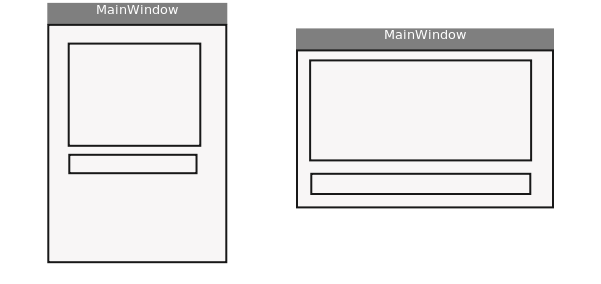
\includegraphics{Figure1.png}   
  \caption{The MainWindow, with a TextEdit and a TextLineEdit, in both
  orientations.}
\end{figure}

\begin{figure}[H]
  \centering
     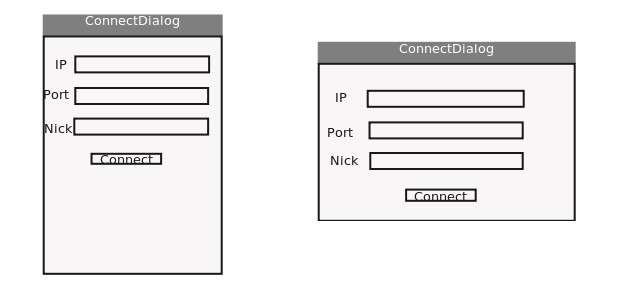
\includegraphics{Figure2.png}
  \caption{The ConnectDialog, with three QLabels, three TextEdits and a button, in both
  orientations.}
\end{figure}

\begin{figure}[H]
  \centering
     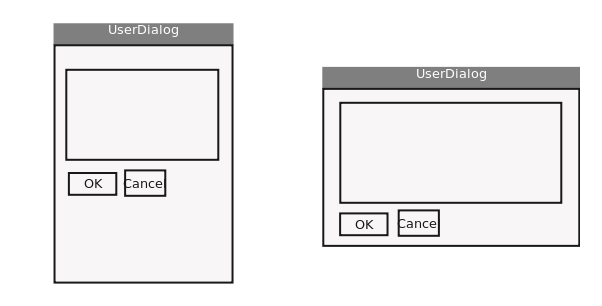
\includegraphics{Figure3.png}
  \caption{The UserDialog, with a TextEdit and two buttons, in both
  orientations.}
\end{figure}


\subsection{Base Classes}

\begin{description}
\item[ConnectDialog] \hfill \\
ConnectDialog, a subclass of QDialog, is a pop-up dialog that appears on program start up. This dialog has three fields: IP, Port, and Nick. Where IP is the IP address of the server, Port is the port teh server is broadcasting over and lastly Nick is the alias the current client window will take upon connecting to the specifed server. Lastly there is a "Connect" button that sends the connection data to the server.

\item[PhoneClient] \hfill \\
PhoneClient, an extension of QThread, is the class that handles all of the communications to teh server. 

\item[MainWindow] \hfill \\
MainWindow, an extension of QMainWindow, is the main application window for the phone client.

\item[UsersDialog] \hfill \\
UsersDialog, a subclass of QDialog, is a pop-up dialog that displays the current users on the server ther client is connected to. It does this by taking in a QStringList via the constructor. Then displays the contents of the list onto the GUI.

\item[ChatServerThread] \hfill \\
ChatServerThread, a subclass of QThread, 

\item[ChatServer] \hfill \\
ChatServer, a subclass of QTcpServer, 

\end{description}

\section{Responsibilities}
Via created the test server pragram while Burns and Chwalowski slpit up the client prgram. More specifically Burns created the Users Window using QT creator. He also helped integrate the different GUI elements together. Lastly he wrote up the documentation for the group's wiki page. 

Chwalowski worked on the connection screen and the main window of the chat client. She also worked on the communications from client to server.Via also worked on the client side communications with Chwalowski.

\section{Problems}
Another  smaller issue was getting TCP to work correctly. Redirection wouldn't work until we waited for input.

One major problem  was when trying to establish a connection with Professor Plassman's server. Our client would connect to the server just fine. Until the users window was opened, in which case the messages we typed in would not be sent and therefore not displayed. The user window would also disrupt recieving other people's messages.  

\end{document}
